\documentclass[pdflatex,sn-mathphys-num]{sn-jnl}
\usepackage{graphicx,amsmath,amssymb,booktabs,siunitx,xcolor,manyfoot}
\renewcommand{\thetable}{S\arabic{table}}
\renewcommand{\thefigure}{S\arabic{figure}}
\renewcommand{\thesection}{S\arabic{section}}
\raggedbottom
\begin{document}
\title[Supplementary Information]{Supplementary Information for ``Parity degeneracy and probe-time anti-resonances in neutral-atom quantum reservoir computing''}
\author*[1]{\fnm{Juan P.} \sur{Rubio}}\email{jprubioo@libertadores.edu.co}
\author[1]{\fnm{Richard G.} \sur{Avella}}
\author[1]{\fnm{Luisa F.} \sur{Ben\'itez}}
\author[2]{\fnm{Sindy J.} \sur{Higuera}}
\affil*[1]{\orgdiv{Department of Aeronautical Engineering}, \orgname{Fundaci\'on Universitaria Los Libertadores}, \orgaddress{\city{Bogot\'a}, \country{Colombia}}}
\affil[2]{\orgname{Instituto Nacional de Metrolog\'ia de Colombia (INM)}, \orgaddress{\city{Bogot\'a}, \country{Colombia}}}
\abstract{This document collects the checks referred to in the main text. Every number and figure is regenerated by \texttt{supplement/make\_supplement.py} from the cached embeddings and hardware records of the public repository; no emulation or hardware access is required. Section and equation references without the prefix S refer to the main text.}
\maketitle

\section{Protocol-design record}\label{sec:s1}

The evaluation protocol of Sec.~3 was not fixed in its first form. Two changes to the readout were made after an initial analysis showed they altered the comparison, and both were applied to every model. Table~\ref{tab:s1} documents their effect on the first three noise seeds, the configuration in which they were found.

First, the degree-2 NG-RC baseline originally used a fixed ridge penalty $\alpha=10^{-4}$. With 45 polynomial features and 44 training anchors this leaves the fit essentially unregularized, and the skill was $-$8.912; selecting the penalty by cross-validation raises it to 0.405. A fixed-penalty baseline would therefore have been an artificially weak comparator. Second, the QRC readout originally used the same fixed penalty. Cross-validation changes the QRC skill by up to $0.7$ at individual total times and removes the deep negative excursions of the total-time sweep, which were an artifact of under-regularization against 500-shot noise rather than a property of the reservoir. Since then, every readout in the study, quantum or classical, selects its penalty by cross-validation on the training anchors. The classical menu was further extended with degree-3 NG-RC and the dimension-matched random-feature control before the six-seed analysis of the main text.

\begin{table}[htb]
\caption{Effect of the readout regularization, base geometry, first three noise seeds. Brackets: 95\% bootstrap intervals. Linear ridge (CV): 0.706.}\label{tab:s1}
\begin{tabular}{@{}lc@{}}
\toprule
Classical model & Skill \\
\midrule
NG-RC deg 2, fixed $\alpha=10^{-4}$ & $-$8.912 [$-$12.190, $-$6.204] \\
NG-RC deg 2, CV & 0.405 [0.301, 0.497] \\
linear ridge, CV & 0.706 [0.653, 0.755] \\
\botrule
\end{tabular}

\vspace{6pt}
\begin{tabular}{@{}ccc@{}}
\toprule
$t_{\mathrm{tot}}$ (\si{\micro\second}) & QRC, fixed $\alpha=10^{-4}$ & QRC, CV \\
\midrule
1.0 & 0.561 [0.475, 0.632] & 0.691 [0.628, 0.744] \\
1.5 & $-$0.597 [$-$1.118, $-$0.143] & $-$0.035 [$-$0.280, 0.177] \\
2.0 & 0.496 [0.344, 0.611] & 0.665 [0.559, 0.751] \\
2.5 & $-$0.288 [$-$0.579, $-$0.046] & 0.097 [$-$0.108, 0.273] \\
3.0 & $-$0.639 [$-$1.007, $-$0.326] & 0.084 [$-$0.020, 0.181] \\
\botrule
\end{tabular}
\end{table}

\section{Degree-3 NG-RC regularization}\label{sec:s2}

Degree-3 NG-RC maps the 8-dimensional window to 165 polynomial features, fitted to 44 training anchors, and its skill in the base geometry is $-$1.691. Table~\ref{tab:s2} shows that this collapse is not a failure of the penalty search. The cross-validated penalty lies in the interior of the default grid for every seed and horizon, and extending the grid by five decades in either direction leaves both the selected penalties and the skill unchanged. Standardizing the polynomial features after expansion, so that the ridge penalty acts uniformly on them, improves the skill only to $-$0.823. The collapse is a small-sample effect; with 80 or more training anchors (fixed-test geometry, Fig.~5) degree-3 NG-RC becomes the strongest classical model.

\begin{table}[htb]
\caption{Degree-3 NG-RC, base geometry, six seeds: pooled skill and the cross-validated ridge penalty over the 18 seed--horizon fits.}\label{tab:s2}
\begin{tabular}{@{}lccc@{}}
\toprule
Variant & Skill & Median $\alpha$ & Range of $\alpha$ \\
\midrule
default grid 1e-3--1e3 & $-$1.691 & 1 & 0.316--316 \\
grid extended 5 decades up, 1e-3--1e8 & $-$1.691 & 1 & 0.316--316 \\
grid extended 5 decades down, 1e-8--1e3 & $-$1.691 & 1 & 0.316--316 \\
standardized polynomial features & $-$0.823 & 2.08 & 0.1--31.6 \\
\botrule
\end{tabular}
\end{table}

\section{Per-state skill and representative predictions}\label{sec:s3}

The preregistered score averages the squared error over the predicted state components before pooling (Sec.~3.2), so each component contributes in proportion to the size of its increments. Table~\ref{tab:s3} resolves the headline comparison ($t_{\mathrm{tot}}=\SI{1.0}{\micro\second}$, 8 atoms, six seeds) by state and horizon. The plunge displacement $\xi$ carries 91\% of the persistence error and therefore dominates the pooled score. It is the only state on which the reservoir matches or exceeds linear ridge; for the pitch $\alpha$ and both velocities the reservoir is clearly behind, and at $H=\tau_c$ its pitch skill is negative. Averaging the per-state skills with equal weight instead gives 0.521 for QRC against 0.727 for linear ridge, a wider gap than the preregistered pooled comparison ($0.698$ against $0.714$). Figure~\ref{fig:s3} shows representative predictions for pitch and plunge on the test block.

\begin{table}[htb]
\caption{Skill by predicted state and horizon, QRC / linear ridge (base geometry, $t_{\mathrm{tot}}=\SI{1.0}{\micro\second}$, six seeds). Share: fraction of the pooled persistence error carried by each state.}\label{tab:s3}
\begin{tabular}{@{}lccccc@{}}
\toprule
State & Share (\%) & $H=\tau_c$ & $2\tau_c$ & $3\tau_c$ & Pooled \\
\midrule
$\alpha$ & 8.8 & $-$0.15 / 0.57 & 0.45 / 0.76 & 0.72 / 0.81 & 0.44 / 0.74 \\
$\dot\alpha$ & 0.2 & 0.56 / 0.78 & 0.61 / 0.77 & 0.10 / 0.40 & 0.45 / 0.67 \\
$\xi$ & 90.6 & 0.79 / 0.95 & 0.78 / 0.81 & 0.68 / 0.62 & 0.73 / 0.71 \\
$\dot\xi$ & 0.5 & 0.43 / 0.75 & 0.39 / 0.71 & 0.54 / 0.85 & 0.47 / 0.79 \\
\botrule
\end{tabular}
\end{table}

\begin{figure}[htb]
\centering
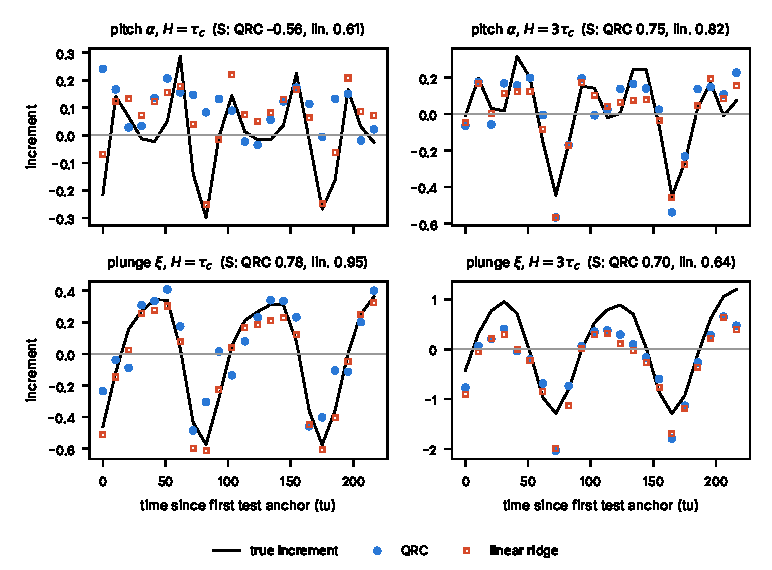
\includegraphics[width=\textwidth]{figS_predictions.pdf}
\caption{Predicted and true finite-horizon increments of pitch and plunge on the 22 test anchors, seed 1234, $t_{\mathrm{tot}}=\SI{1.0}{\micro\second}$. Titles give the per-panel skill for this seed.}\label{fig:s3}
\end{figure}

\section{Twelve-atom target definition}\label{sec:s4}

The 12-atom configuration of Table~7 encodes all six states and predicts all six, whereas the 8- and 16-atom configurations predict the four mechanical states. Restricting the 12-atom target to the four mechanical states, with the same embeddings and readout, leaves skill and gap unchanged to the second decimal (Table~\ref{tab:s4}); the auxiliary aerodynamic states contribute negligibly to the pooled error.

\begin{table}[htb]
\caption{Twelve-atom configuration with six-state and four-state targets (first three seeds). Gap: QRC minus best NG-RC (CV) on the same window.}\label{tab:s4}
\begin{tabular}{@{}clccc@{}}
\toprule
$t_{\mathrm{tot}}$ (\si{\micro\second}) & Target & QRC & Best NG-RC & Gap \\
\midrule
1.0 & six states & 0.700 & 0.760 & $-$0.061 \\
1.0 & four mechanical states & 0.700 & 0.760 & $-$0.060 \\
2.0 & six states & 0.592 & 0.760 & $-$0.168 \\
2.0 & four mechanical states & 0.592 & 0.760 & $-$0.168 \\
\botrule
\end{tabular}
\end{table}

\section{Hardware post-selection}\label{sec:s5}

Shots in which any atom failed to load were discarded before computing the hardware embeddings (23.9\% of shots). Atom sorting precedes the encoding pulse, so survival cannot depend on the encoded detunings, but a correlation between survival and the hardware--emulator deviation could still bias the node skill. For each probe we define the mean deviation direction $\hat{\mathbf{u}}=\overline{\mathbf{d}}/\lVert\overline{\mathbf{d}}\rVert$, with $\mathbf{d}_k=E^{\mathrm{hw}}_k-E^{\mathrm{emu,500}}_k$ the deviation of anchor $k$, and project each anchor on it. Table~\ref{tab:s5} shows that the projection is uncorrelated with the surviving shot fraction at every probe; at the node, $r=-0.05$ ($p=0.69$), and anchors above and below the median survival have the same mean projection (0.234 and 0.238).

\begin{table}[htb]
\caption{Surviving shot fraction and its relation to the hardware--emulator deviation (seed 1234). $r$: Pearson correlation between survival and projection, with $p$-value. Proj.: mean projection for anchors above (high) and below (low) the median survival.}\label{tab:s5}
\begin{tabular}{@{}cccccc@{}}
\toprule
$t$ (\si{\micro\second}) & Anchors & Survival [range] & $r$ ($p$) & Proj., high & Proj., low \\
\midrule
0.50 & 65 & 0.779 [0.68, 0.86] & $+$0.058 (0.65) & $+$0.142 & $+$0.095 \\
0.70 & 66 & 0.737 [0.58, 0.87] & $-$0.049 (0.69) & $+$0.234 & $+$0.238 \\
1.80 & 66 & 0.768 [0.67, 0.88] & $-$0.042 (0.74) & $+$0.180 & $+$0.156 \\
\botrule
\end{tabular}
\end{table}

\section{Waveform amendment}\label{sec:s6}

Aquila requires the drive and the detuning to start and end at zero, so the constant quench of the emulator cannot be run directly. Before submission, the programmed waveforms were executed on Braket's local, noise-free analog Hamiltonian simulator with the same program and parsing as the hardware path (100 shots, seed 1234). The submitted waveform E1 uses \SI{0.05}{\micro\second} linear ramps, set by the slew-rate limit of $250~\mathrm{rad}/\si{\micro\second}^2$ and the \SI{50}{ns} time step, with programmed durations of $t+\SI{0.05}{\micro\second}$ so that the plateau-equivalent time equals the nominal probe. Its embeddings correlate with the 500-shot emulator as closely as two emulator samplings do, with unit slope, and it reproduces the node ($-$0.201). An earlier implementation with ramps of $\min(\SI{0.2}{\micro\second},t/4)$ erased the node (0.661), which would have invalidated the preregistered contrast for reasons unrelated to decoherence (Table~\ref{tab:s6}).

\begin{table}[htb]
\caption{Noise-free simulation of the programmed waveforms. $\rho$: correlation of embeddings with the 500-shot constant-profile emulator; sampling baseline: the same correlation between two emulator samplings (100 and 500 shots); $b$: no-intercept slope onto the emulator.}\label{tab:s6}
\begin{tabular}{@{}lccccc@{}}
\toprule
Waveform & $t$ (\si{\micro\second}) & Skill & $\rho$ & Sampling baseline & $b$ \\
\midrule
E1 (submitted) & 0.50 & 0.666 & 0.971 & 0.968 & 1.001 \\
E1 (submitted) & 0.70 & $-$0.201 & 0.953 & 0.952 & 1.000 \\
E1 (submitted) & 1.80 & $-$0.461 & 0.944 & 0.938 & 0.994 \\
earlier ramp & 0.50 & 0.650 & 0.847 & 0.968 & -- \\
earlier ramp & 0.70 & 0.661 & 0.654 & 0.952 & -- \\
earlier ramp & 1.80 & $-$0.106 & 0.182 & 0.938 & -- \\
\botrule
\end{tabular}
\end{table}

\section{Sign-definite encoding: full grid}\label{sec:s7}

Table~\ref{tab:s7} extends Table~3 of the main text to the full grid of total times and spacings, computed by exact eight-atom evolution with 500-shot resampling (median of ten realizations; Sec.~4.3). Values at $t_{\mathrm{tot}}=\SI{1.0}{\micro\second}$ differ from the Bloqade values of Table~3 by shot noise only.

\begin{table}[htb]
\caption{Pooled skill for both encodings over the full grid (8 atoms, two-probe $Z$, base geometry, six seeds). Brackets: 95\% bootstrap intervals of the median realization.}\label{tab:s7}
\begin{tabular}{@{}lccccc@{}}
\toprule
Encoding & $a$ (\si{\micro\meter}) & $t_{\mathrm{tot}}$ (\si{\micro\second}) & Infinite shots & 500 shots & Worst seed \\
\midrule
symmetric & 10 & 1.0 & 0.705 & 0.696 [0.660, 0.728] & 0.640 \\
symmetric & 10 & 1.5 & $-$0.187 & $-$0.095 [$-$0.322, 0.096] & $-$0.402 \\
symmetric & 10 & 2.0 & 0.645 & 0.673 [0.608, 0.731] & 0.481 \\
symmetric & 10 & 2.5 & $-$0.486 & $-$0.052 [$-$0.213, 0.112] & $-$0.460 \\
symmetric & 10 & 3.0 & 0.139 & 0.120 [0.053, 0.198] & 0.053 \\
symmetric & 30 & 1.0 & $-$0.617 & $-$0.635 [$-$0.677, $-$0.584] & $-$0.796 \\
symmetric & 30 & 1.5 & $-$0.676 & $-$0.667 [$-$0.716, $-$0.618] & $-$0.821 \\
symmetric & 30 & 2.0 & $-$0.764 & $-$0.788 [$-$0.830, $-$0.726] & $-$0.930 \\
symmetric & 30 & 2.5 & $-$0.782 & $-$0.781 [$-$0.830, $-$0.730] & $-$0.856 \\
symmetric & 30 & 3.0 & $-$0.780 & $-$0.784 [$-$0.830, $-$0.735] & $-$0.832 \\
sign-definite & 10 & 1.0 & 0.751 & 0.749 [0.710, 0.788] & 0.707 \\
sign-definite & 10 & 1.5 & 0.002 & $-$0.100 [$-$0.337, 0.109] & $-$0.801 \\
sign-definite & 10 & 2.0 & 0.012 & 0.020 [$-$0.091, 0.140] & $-$0.102 \\
sign-definite & 10 & 2.5 & 0.147 & 0.173 [0.053, 0.291] & 0.087 \\
sign-definite & 10 & 3.0 & $-$0.757 & $-$0.682 [$-$0.913, $-$0.446] & $-$1.229 \\
sign-definite & 30 & 1.0 & 0.748 & 0.744 [0.702, 0.785] & 0.715 \\
sign-definite & 30 & 1.5 & 0.173 & 0.161 [0.057, 0.255] & 0.079 \\
sign-definite & 30 & 2.0 & 0.231 & 0.255 [0.123, 0.362] & $-$0.078 \\
sign-definite & 30 & 2.5 & 0.706 & 0.699 [0.645, 0.750] & 0.645 \\
sign-definite & 30 & 3.0 & 0.170 & 0.168 [0.073, 0.254] & 0.105 \\
\botrule
\end{tabular}
\end{table}

\end{document}
